\textbf{{1.硬盘存储器数据记录方式}}

记录数据的方式主要有6类,但考生只需掌握3种即可,如下图所示。

\textbf{1)归零制(RZ)。}记录``1''时,通正向脉冲电流;记录``0''时,通反向脉冲电流。``0''和``1''信息之间驱动电流归零。

\textbf{2)不归零制(NRZ)。}记录``1''时,通正向脉冲电流;记录``0''时,通反向脉冲电流。只有当相邻信息代码不同时,电流才改变方向,故称为``见变就翻''。

\textbf{3)``见1就翻''的不归零制(NRZ1)。}只有记录``1''时,电流才改变方向,如下图所示。

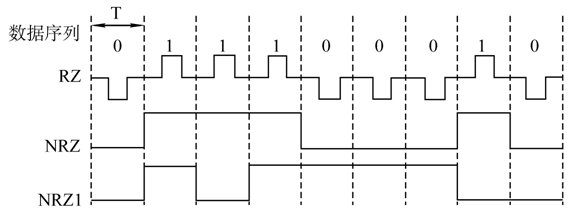
\includegraphics[width=3.65625in,height=1.34375in]{png-jpeg-pics/314EA0D1735F7CA96067628202722D32.png}

\textbf{{2.硬盘存储器的技术指标}}

\textbf{(1)记录密度}

\textbf{记录密度}通常{是指单位长度内所存储的二进制信息量}。硬盘存储器一般需要用道密度和位密度一起来表示。

\textbf{道密度}指磁盘沿半径方向单位长度的磁道数(就是单位长度内有多少个同心圆)。相邻磁道之间的距离称为道距。

\textbf{位密度}(或称线密度)指单位长度磁道能记录二进制信息的位数。

{注意:磁盘的所有磁道记录的信息量一定是相等的,并不是圆越大,记录的信息就越多。既然大圆和小圆记录的信息是一样多,那么每个磁道的位密度都是不同的(很明显,圈越大,位密度越小)。另外,一般题目中给出的磁盘位密度都是指最大位密度,也就是最内层圈的位密度。}

\textbf{(2)存储容量}

存储容量指外存所能存储的二进制信息总数量,以位或字节为单位。以硬盘存储器为例,存储容量可按下式计算:\textbf{C=n×k×s}\\
式中,C为存储总容量;n为存放信息的盘面数;k为每个盘面的磁道数;s为每条磁道上记录的二进制代码数。

\textbf{(3)平均寻址时间}

{平均寻址时间=(最大寻道时间+最小寻道时间)/2+(最大等待时间+最小等待时间)/2}

\textbf{(4)数据传输率}

数据传输率指单位时间内磁表面存储器向主机传输数据的位数或字节数,它与记录密度和磁盘转动的速度有关。

\textbf{(5)误码率}

如果从磁盘读出N位数据,有M位出错,那么误码率为M/N。为了减少误码率,硬盘存储器通常采用循环冗余码来校验数据。

\textbf{{3.磁盘阵列}}

\textbf{RAID指由多个小容量磁盘代替一个大容量的磁盘。}

\textbf{1)RAID
0。}最简单的磁盘阵列架构。写入时将资料分成数个小块,再同时送到不同的磁盘内存储,读取资料时也需要从不同的磁盘内读取,然后重新组合。正是由于RAID将资料分块存储,使得存储速度大大加快。它的缺点也显而易见,如果某一个磁盘的数据损坏,将会因资料不完整而无法读取,造成系统停止,甚至毁掉所有硬盘资料。

\textbf{2)RAID
1。又称为镜像备份,}意思就是可以将资料如镜子里的成像一样,在两个硬盘上各保持一份完全相同的备份,使得资料完全一样。写入时,相同的资料会同时写到磁盘阵列中的每一个磁盘;读取时仅从其中一个读取即可。由于每个硬盘都有一个镜像的硬盘,因此当某个硬盘出现损坏,并不会影响整个系统的运行。可以说RAID
1的容错性是相当好的。

\textbf{{4.光盘存储器}}

\textbf{(1)只读型光盘}

只读型光盘内的数据和程序由厂家事先写入,用户只能读出,不能修改或写入新的内容。非常类似于ROM的特性,故又将其称为CD-ROM。

\textbf{(2)只写一次型光盘}

只写一次型光盘允许用户写入信息,写入后可多次读出,但不能再修改,故称其为``写一次型''。

\textbf{(3)可擦写型光盘}

可擦写型光盘由于是激光照射在磁性介质上进行读/写,因为这种光盘类似于磁盘,可以重复读写。
